\section{Esempi}\vspace{-0.3em}
\lstinputlisting[style=armasmstyle]{code/64_bit_addition.s}\vspace{-0.6em}
\lstinputlisting[style=armasmstyle]{code/64_bit_subtraction.s}

\begin{minipage}{0.7\columnwidth}
    \lstinputlisting[style=armasmstyle]{code/64_bit_shift.s}
\end{minipage}
\begin{minipage}{0.3\columnwidth}
    \centering
    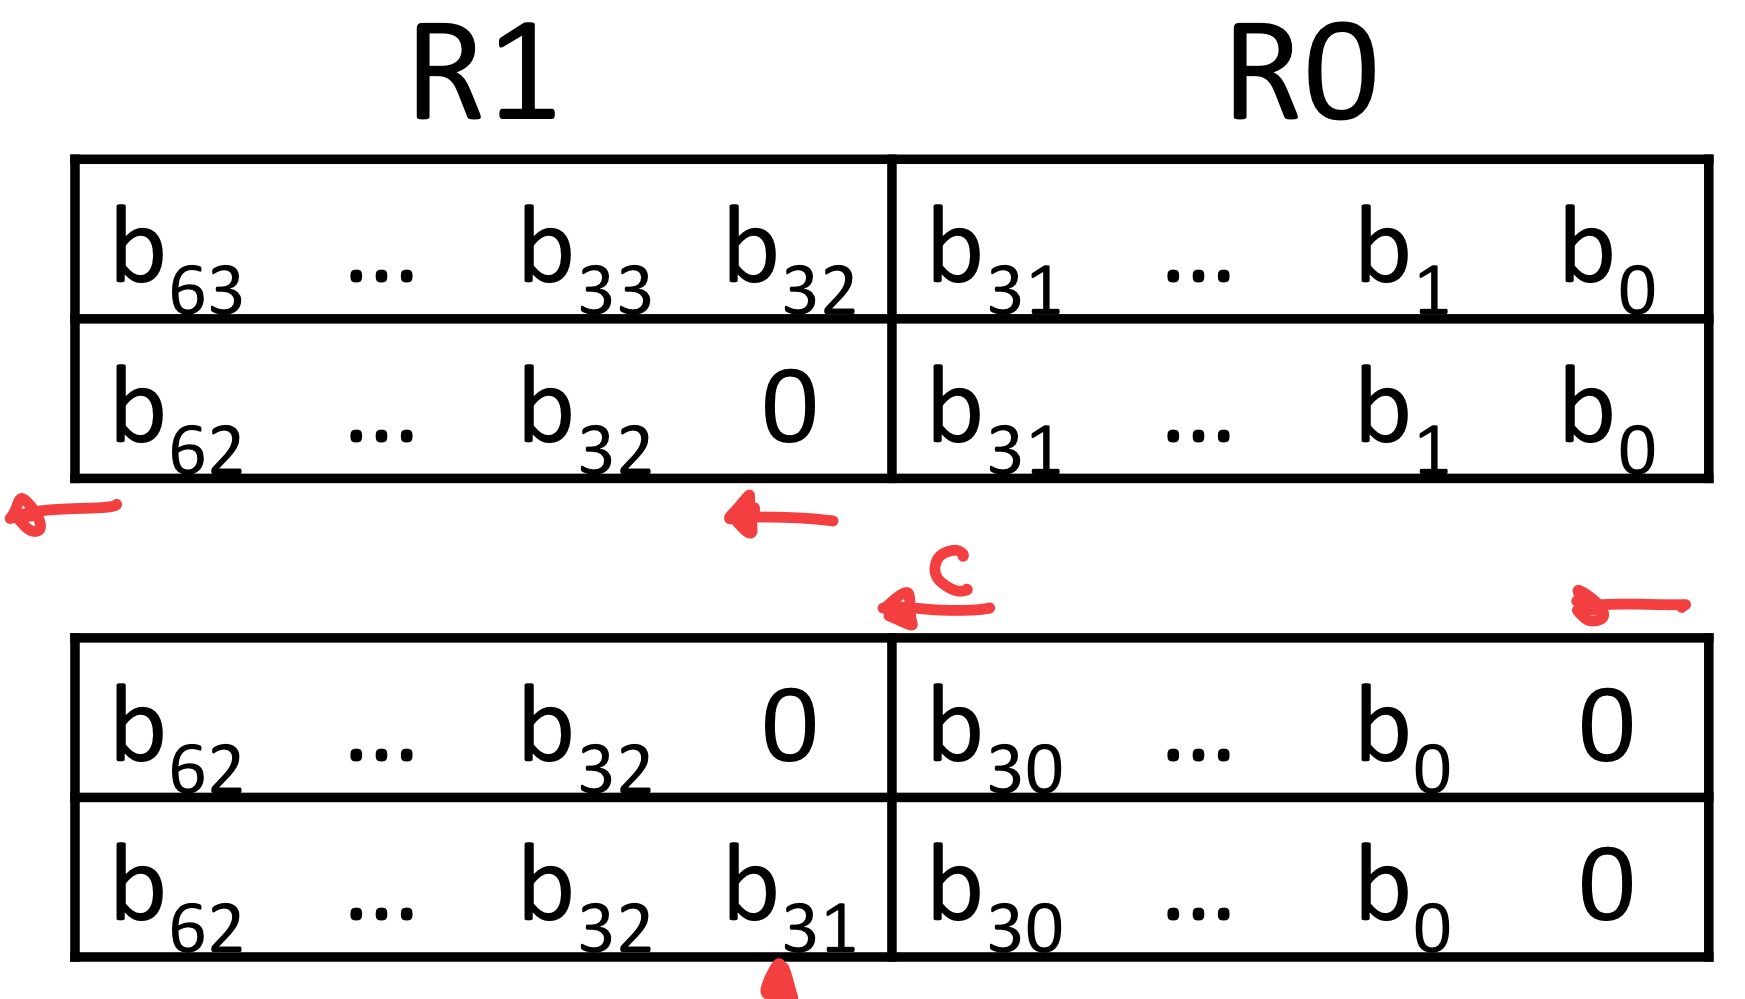
\includegraphics[width=\linewidth]{images/64_bit_shift.png}\medbreak
    Equivalente a: ($\cdot 2$)
\end{minipage}

% --- ESEMPIO 1 ---
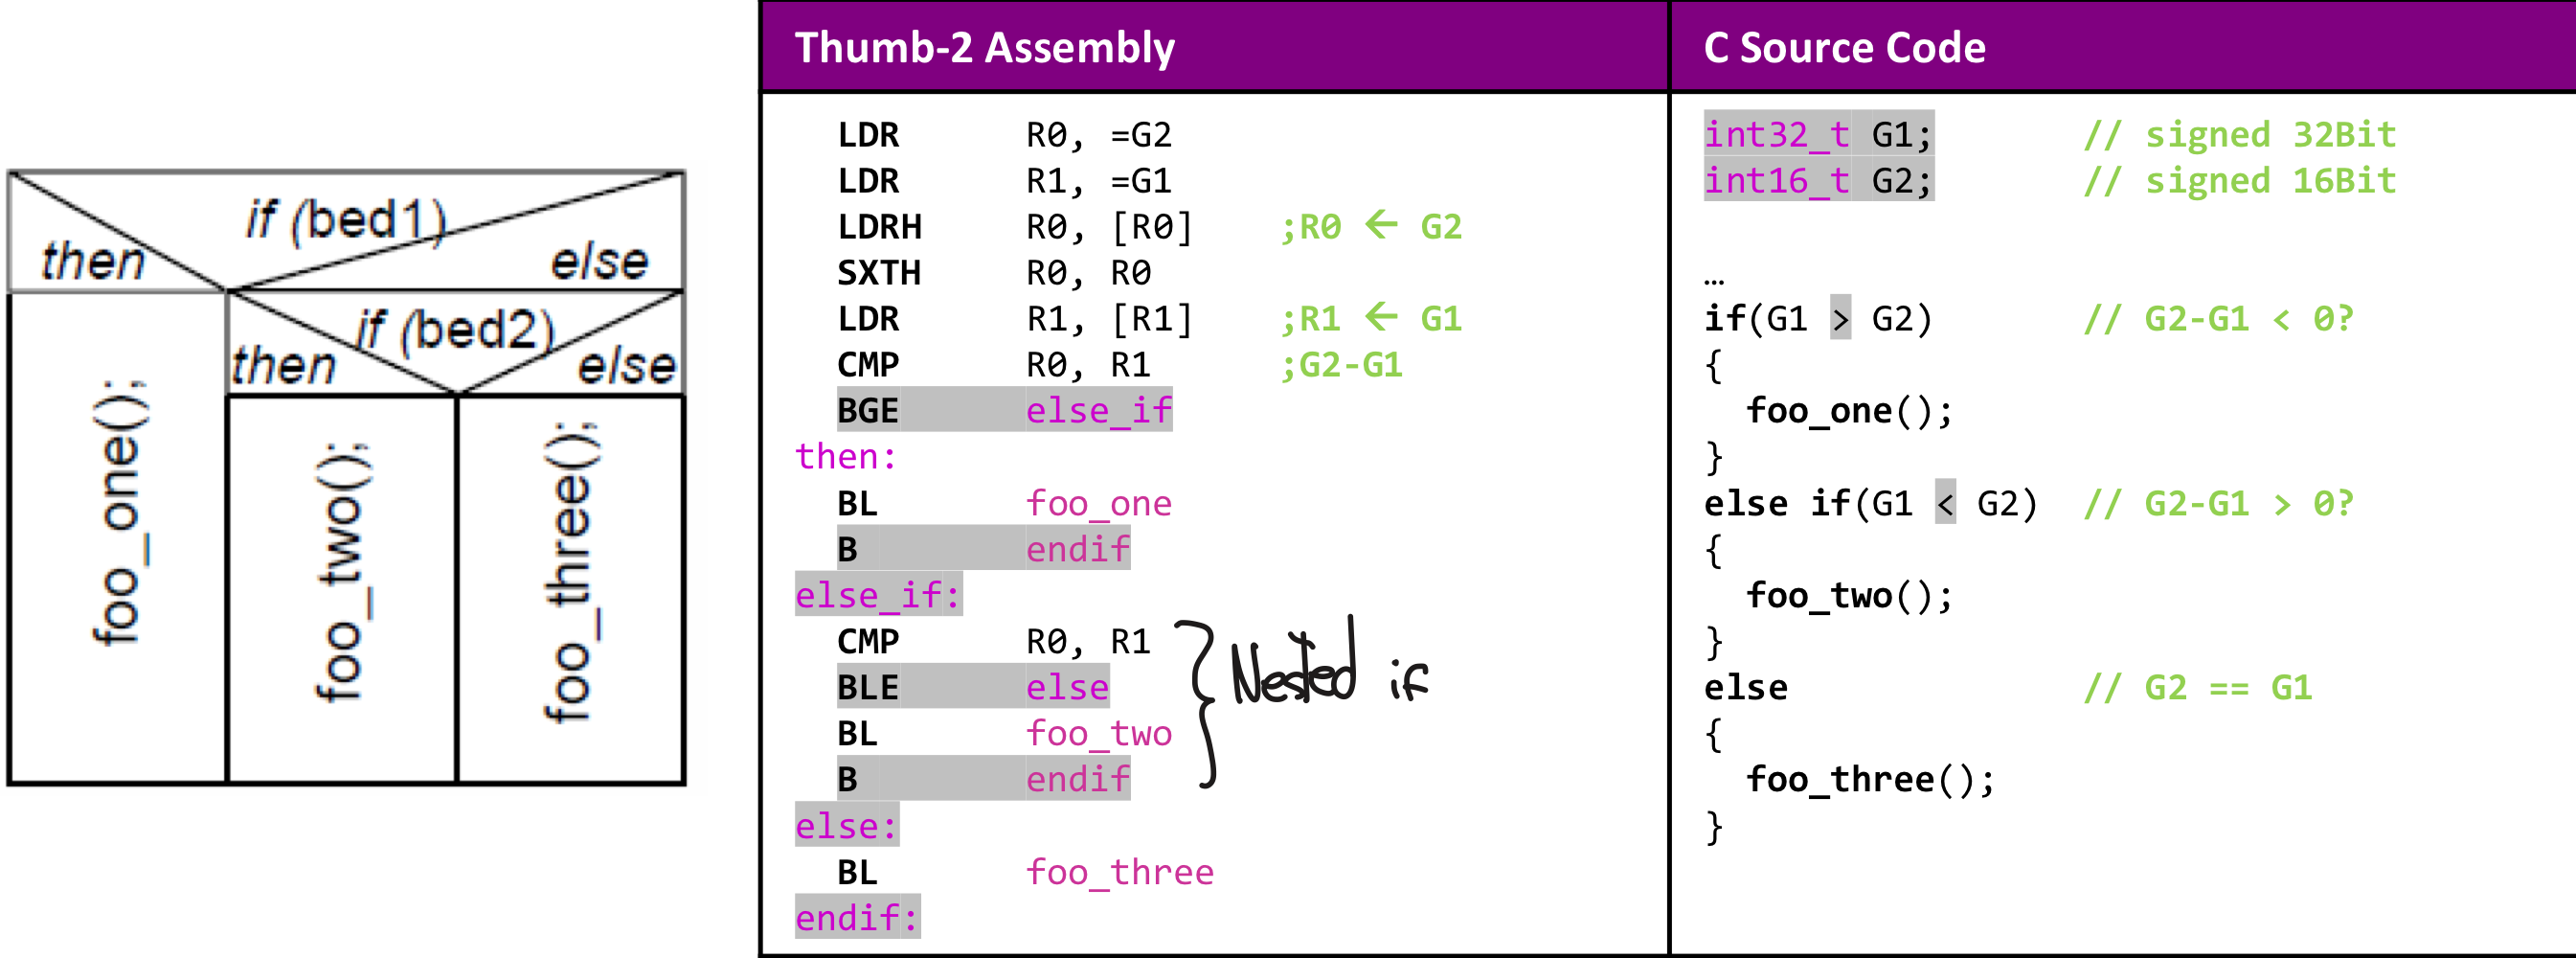
\includegraphics[width=\linewidth]{images/if_if_else.png}
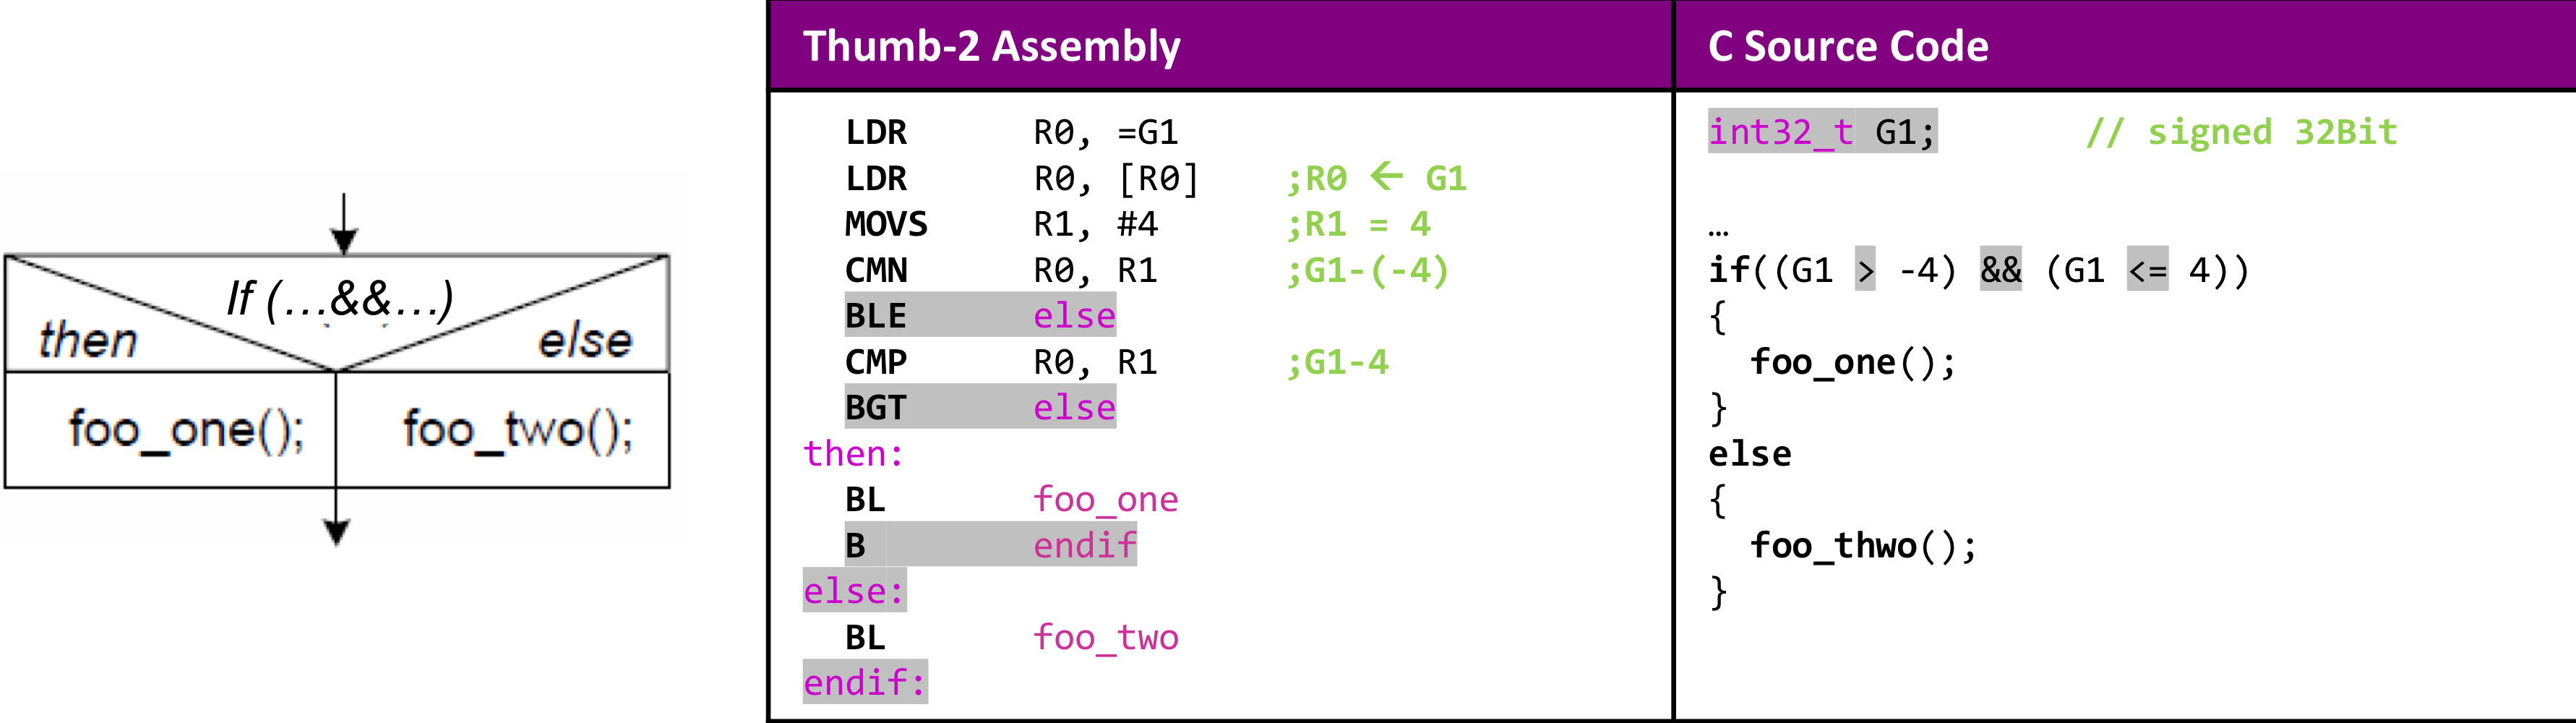
\includegraphics[width=\linewidth]{images/if_and_and.png}
% \noindent
% \begin{minipage}[t]{0.25\columnwidth}
%     \vspace{0pt} % Forza l'allineamento in alto
%     \centering
%     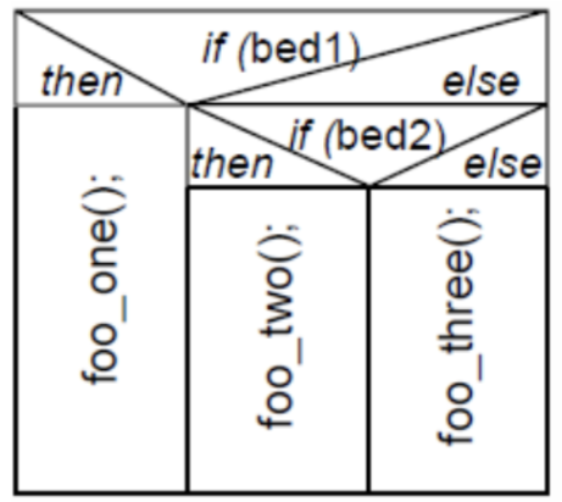
\includegraphics[width=\linewidth]{images/triple_if_else.png}
% \end{minipage}% <-- Il % previene spazi orizzontali extra
% \hfill
% \begin{minipage}[t]{0.72\columnwidth}
%     \vspace{0pt}
%     \setlength{\fboxsep}{2pt} % Riduce l'altezza del box viola
    
%     \begin{minipage}[t]{0.48\textwidth}
%         \colorbox{sectioncolor}{\makebox[\dimexpr\linewidth-2\fboxsep\relax]{\footnotesize\textbf{\color{white}Thumb-2 Assembly}}}
%         \lstinputlisting[style=armasmstyle, basicstyle=\footnotesize\ttfamily, aboveskip=2pt, belowskip=0pt]{code/beispiel_1.s}
%     \end{minipage}%
%     \hspace{0.04\textwidth}%
%     \begin{minipage}[t]{0.48\textwidth}
%         \colorbox{sectioncolor}{\makebox[\dimexpr\linewidth-2\fboxsep\relax]{\color{white}\footnotesize\textbf{C Source Code}}}
%         \lstinputlisting[language=C, basicstyle=\footnotesize\ttfamily, aboveskip=1pt, belowskip=0pt]{code/beispiel_1.c}
%     \end{minipage}
% \end{minipage}

\vspace{1ex} % Spazio ridotto tra i due esempi

% --- ESEMPIO 2 ---
% \noindent
% \begin{minipage}[t]{0.25\columnwidth}
%     \vspace{0pt}
%     \centering
%     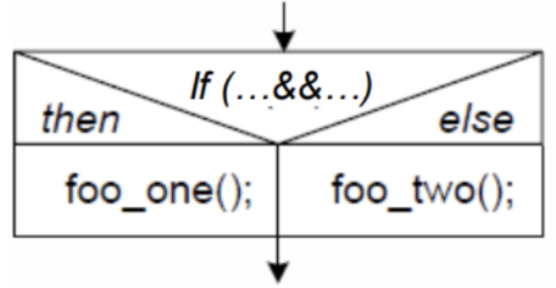
\includegraphics[width=\linewidth]{images/if_else.png}
% \end{minipage}%
% \hfill
% \begin{minipage}[t]{0.72\columnwidth}
%     \vspace{0pt}
%     \setlength{\fboxsep}{2pt}
    
%     \begin{minipage}[t]{0.48\textwidth}
%         \colorbox{sectioncolor}{\makebox[\dimexpr\linewidth-2\fboxsep\relax]{\footnotesize\textbf{\color{white}Thumb-2 Assembly}}}
%         \lstinputlisting[style=armasmstyle, basicstyle=\footnotesize\ttfamily, aboveskip=2pt, belowskip=0pt]{code/beispiel_2.s}
%     \end{minipage}%
%     \hspace{0.04\textwidth}%
%     \begin{minipage}[t]{0.48\textwidth}
%         \colorbox{sectioncolor}{\makebox[\dimexpr\linewidth-2\fboxsep\relax]{\footnotesize\textbf{\color{white}C Source Code}}}
%         \lstinputlisting[language=C, basicstyle=\footnotesize\ttfamily, aboveskip=1pt, belowskip=0pt]{code/beispiel_2.c}
%     \end{minipage}
% \end{minipage}

\begin{center}
    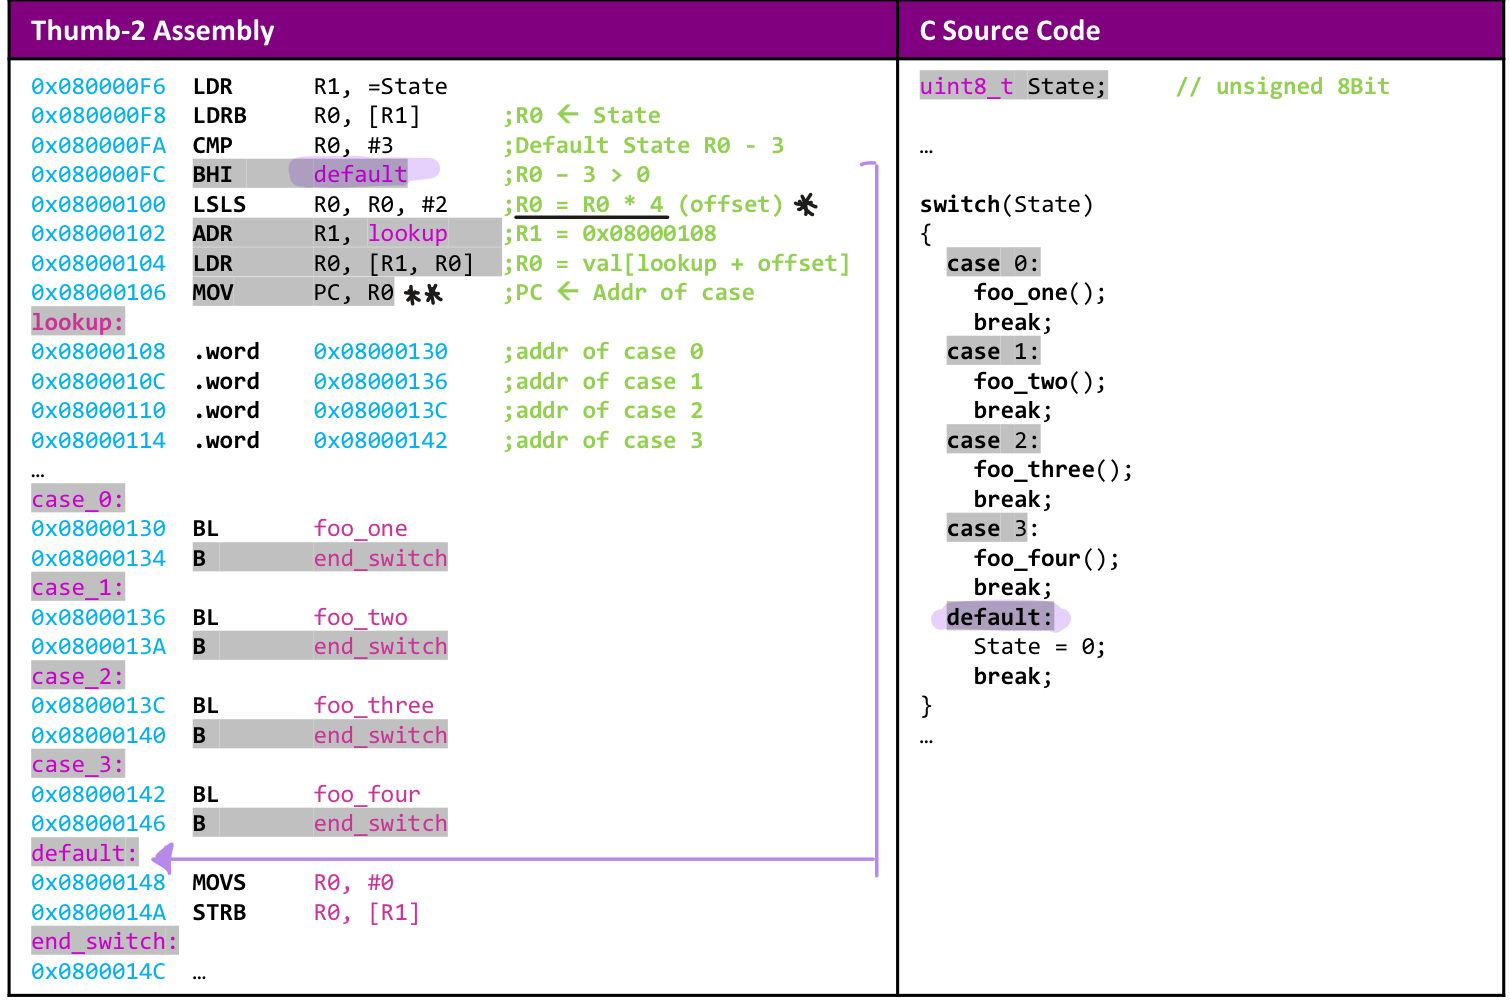
\includegraphics[width=0.9\linewidth]{images/switch_case.png}
\end{center}

\begin{enumerate}
    \item \textbf{Controllo limiti:} Verifica valore di \texttt{State} per saltare subito al \texttt{default} se l'indice è fuori range.
    \item \textbf{Calcolo offset:} Moltiplicazione del valore per 4 ($State \ll 2$) tramite shift logico, poiché ogni puntatore nella look-up table occupa 32 bit (4 byte).
    \item \textbf{Recupero puntatore:} Lettura dell'indirizzo di destinazione esatto sommando l'offset calcolato all'indirizzo base della tabella.
    \item \textbf{Branch:} avviare l'esecuzione del caso specifico.
\end{enumerate}


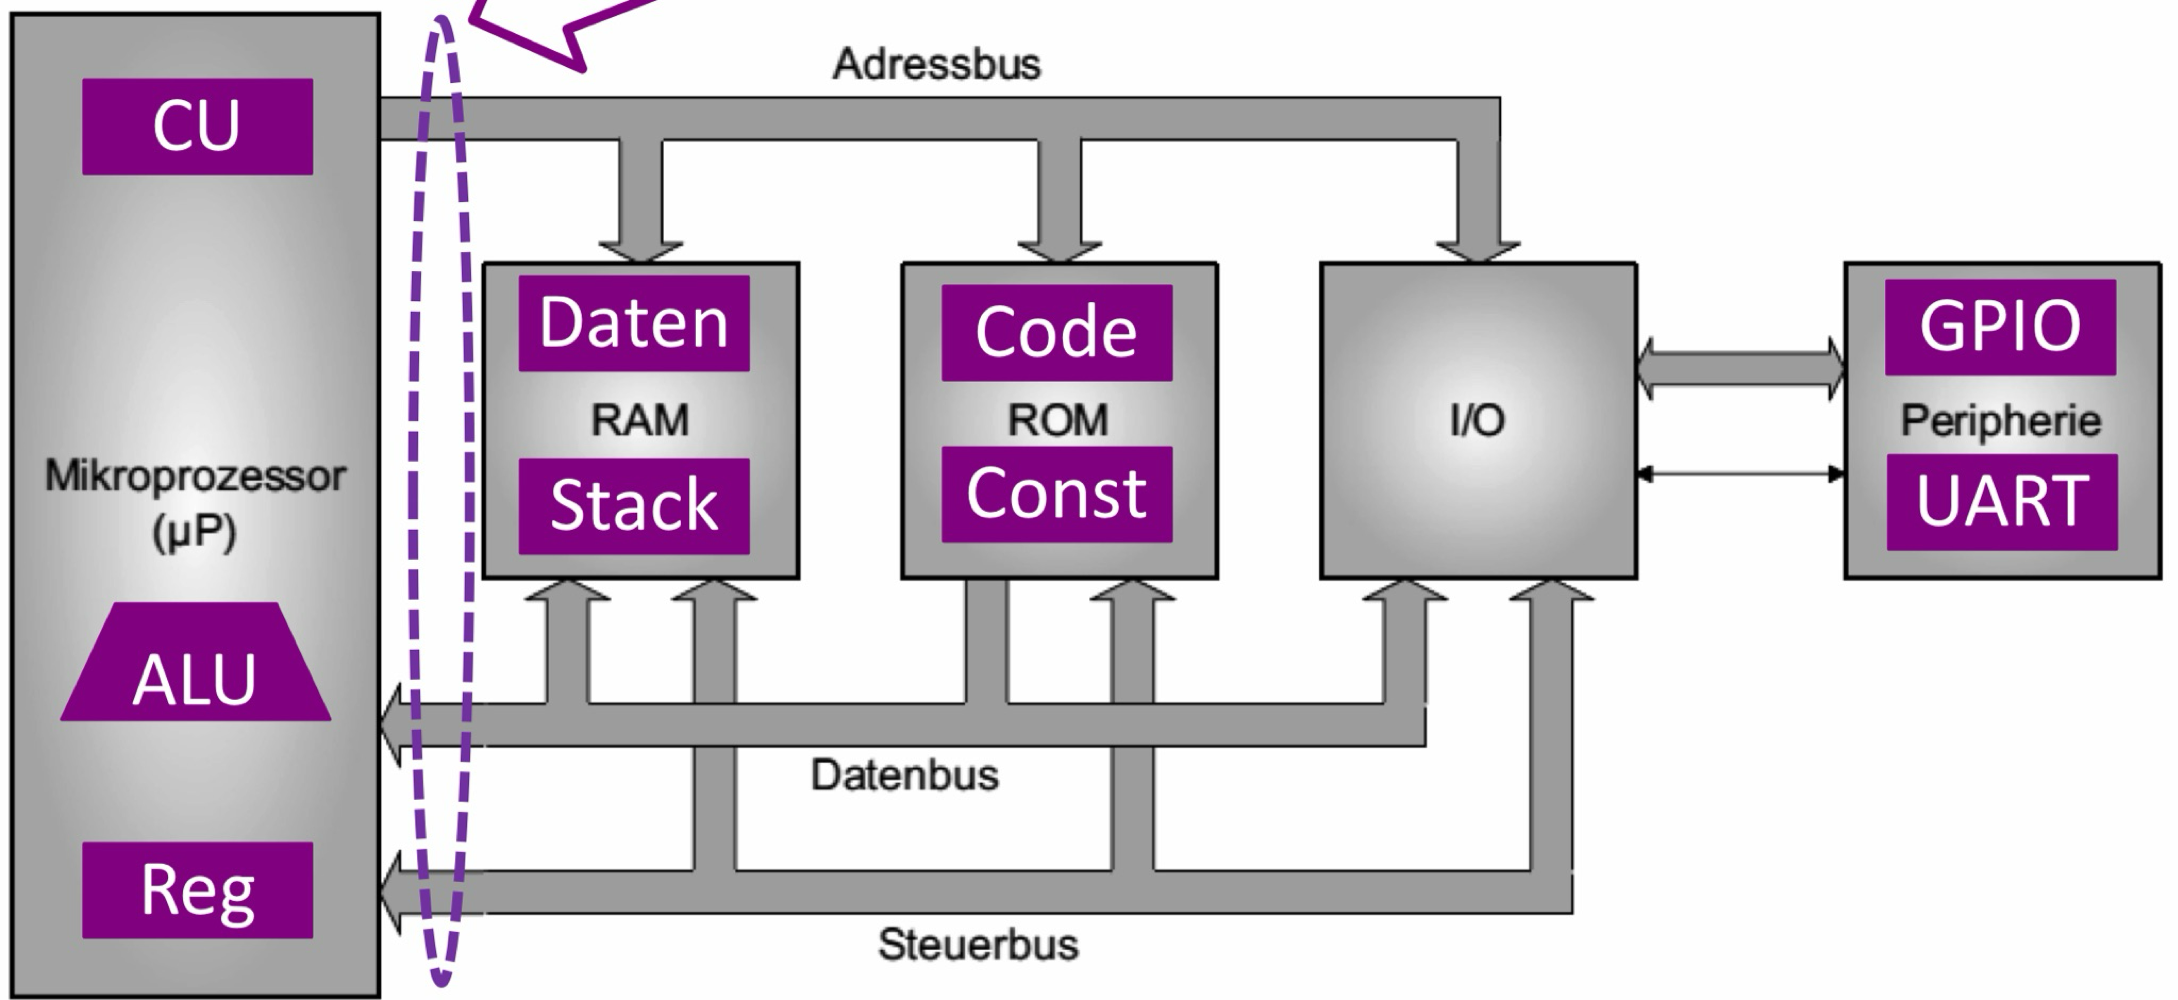
\includegraphics[width=0.75\linewidth]{images/microprocessor.png}

\begin{minipage}{0.6\linewidth}
    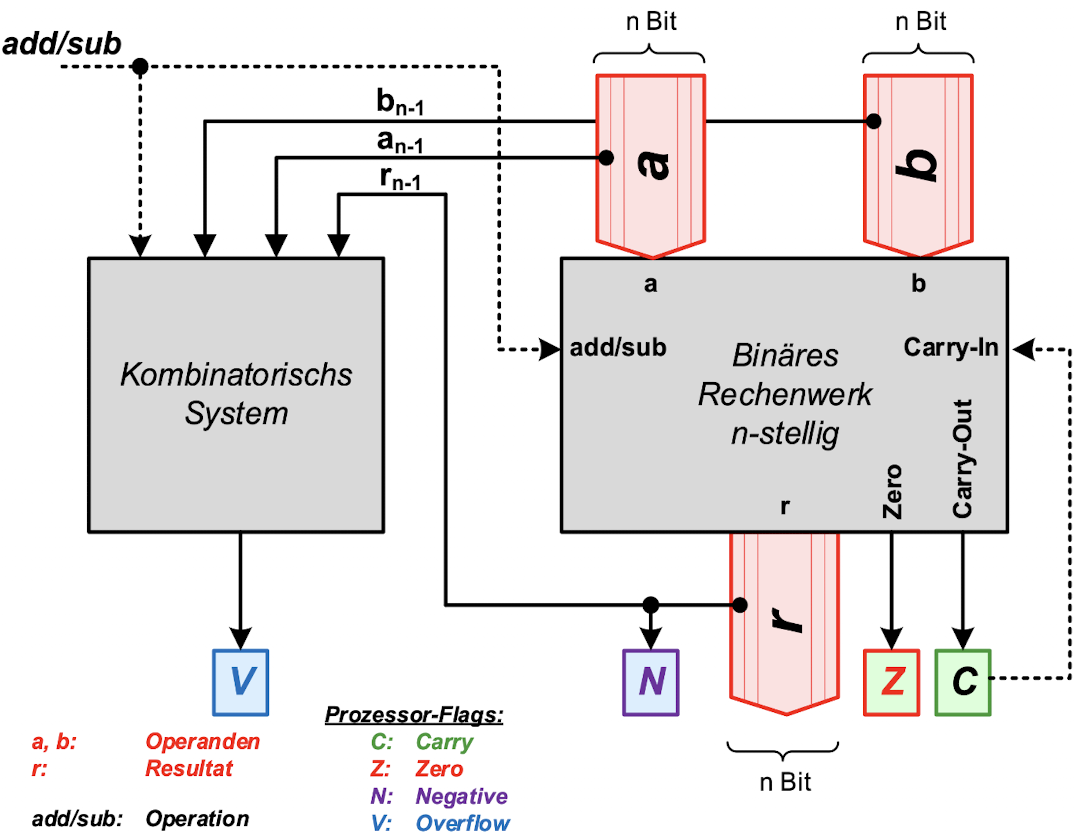
\includegraphics[width = \linewidth]{images/duales_alu.png}
    \hrule
\end{minipage}
\hfill\vline\hfill
\begin{minipage}{0.3\linewidth}
    \rotatebox{90}{%
    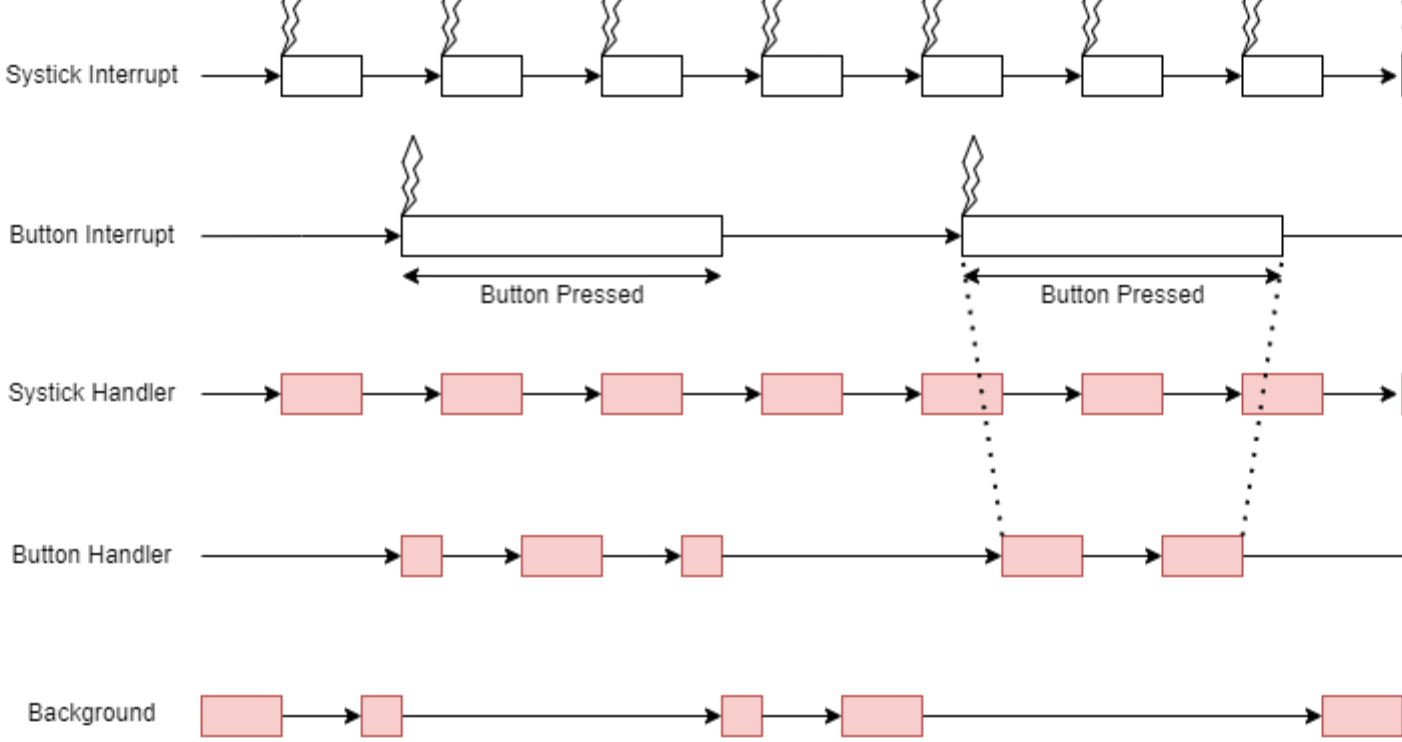
\includegraphics[width = 1.7\linewidth]{images/isr_priorities_2.png}}
\end{minipage}

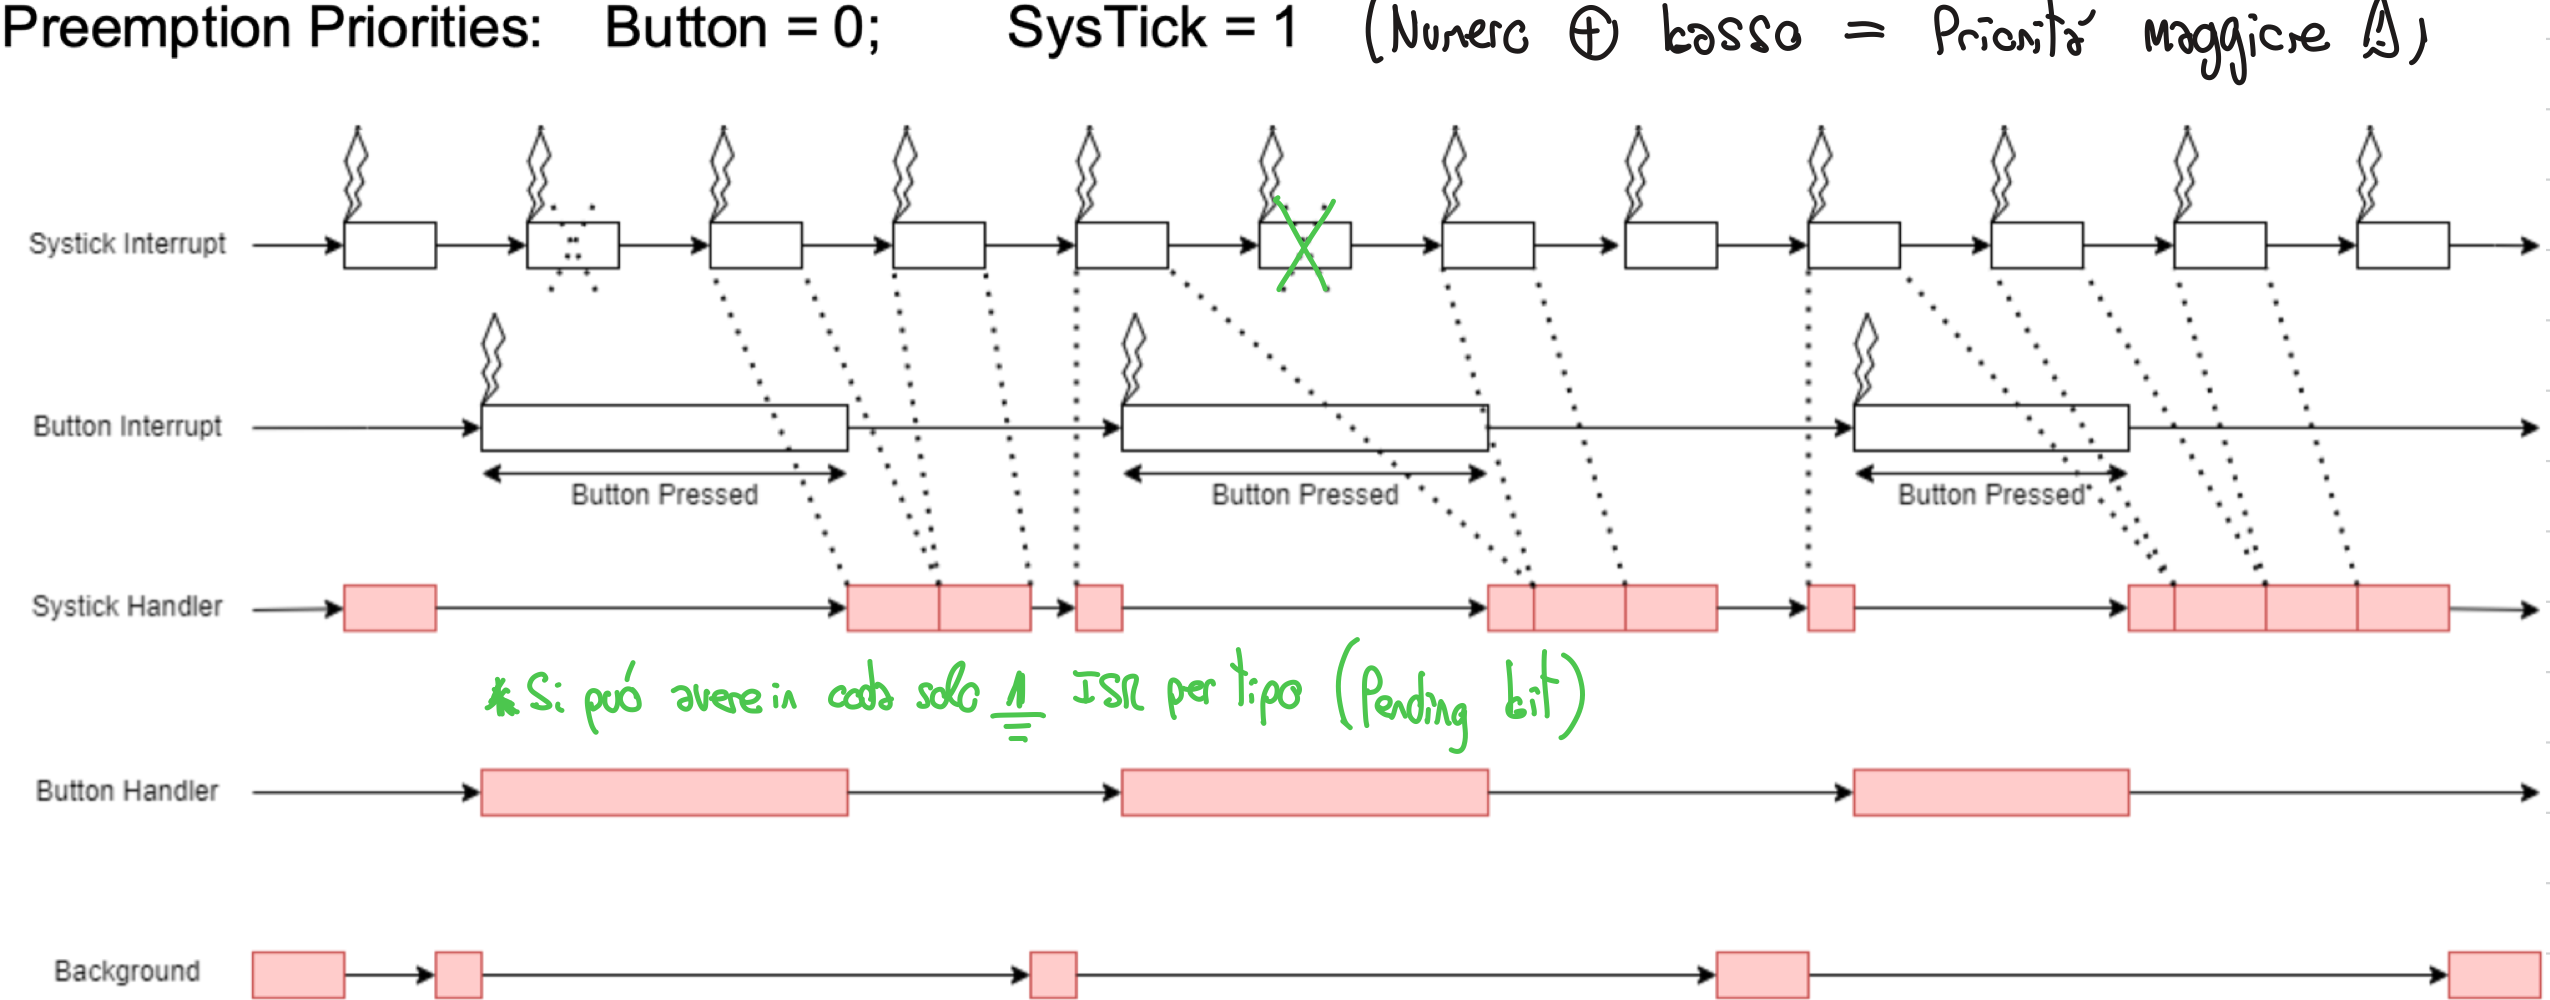
\includegraphics[width = 0.9\linewidth]{images/isr_priorities.png}
